\documentclass[12pt]{article}\usepackage[]{graphicx}\usepackage[]{color}
% maxwidth is the original width if it is less than linewidth
% otherwise use linewidth (to make sure the graphics do not exceed the margin)
\makeatletter
\def\maxwidth{ %
  \ifdim\Gin@nat@width>\linewidth
    \linewidth
  \else
    \Gin@nat@width
  \fi
}
\makeatother

\definecolor{fgcolor}{rgb}{0.345, 0.345, 0.345}
\newcommand{\hlnum}[1]{\textcolor[rgb]{0.686,0.059,0.569}{#1}}%
\newcommand{\hlstr}[1]{\textcolor[rgb]{0.192,0.494,0.8}{#1}}%
\newcommand{\hlcom}[1]{\textcolor[rgb]{0.678,0.584,0.686}{\textit{#1}}}%
\newcommand{\hlopt}[1]{\textcolor[rgb]{0,0,0}{#1}}%
\newcommand{\hlstd}[1]{\textcolor[rgb]{0.345,0.345,0.345}{#1}}%
\newcommand{\hlkwa}[1]{\textcolor[rgb]{0.161,0.373,0.58}{\textbf{#1}}}%
\newcommand{\hlkwb}[1]{\textcolor[rgb]{0.69,0.353,0.396}{#1}}%
\newcommand{\hlkwc}[1]{\textcolor[rgb]{0.333,0.667,0.333}{#1}}%
\newcommand{\hlkwd}[1]{\textcolor[rgb]{0.737,0.353,0.396}{\textbf{#1}}}%
\let\hlipl\hlkwb

\usepackage{framed}
\makeatletter
\newenvironment{kframe}{%
 \def\at@end@of@kframe{}%
 \ifinner\ifhmode%
  \def\at@end@of@kframe{\end{minipage}}%
  \begin{minipage}{\columnwidth}%
 \fi\fi%
 \def\FrameCommand##1{\hskip\@totalleftmargin \hskip-\fboxsep
 \colorbox{shadecolor}{##1}\hskip-\fboxsep
     % There is no \\@totalrightmargin, so:
     \hskip-\linewidth \hskip-\@totalleftmargin \hskip\columnwidth}%
 \MakeFramed {\advance\hsize-\width
   \@totalleftmargin\z@ \linewidth\hsize
   \@setminipage}}%
 {\par\unskip\endMakeFramed%
 \at@end@of@kframe}
\makeatother

\definecolor{shadecolor}{rgb}{.97, .97, .97}
\definecolor{messagecolor}{rgb}{0, 0, 0}
\definecolor{warningcolor}{rgb}{1, 0, 1}
\definecolor{errorcolor}{rgb}{1, 0, 0}
\newenvironment{knitrout}{}{} % an empty environment to be redefined in TeX

\usepackage{alltt}\usepackage[]{graphicx}\usepackage[]{color}
%% maxwidth is the original width if it is less than linewidth
%% otherwise use linewidth (to make sure the graphics do not exceed the margin)
\makeatletter
\def\maxwidth{ %
  \ifdim\Gin@nat@width>\linewidth
    \linewidth
  \else
    \Gin@nat@width
  \fi
}
\makeatother

\definecolor{fgcolor}{rgb}{0.345, 0.345, 0.345}
\newcommand{\hlnum}[1]{\textcolor[rgb]{0.686,0.059,0.569}{#1}}%
\newcommand{\hlstr}[1]{\textcolor[rgb]{0.192,0.494,0.8}{#1}}%
\newcommand{\hlcom}[1]{\textcolor[rgb]{0.678,0.584,0.686}{\textit{#1}}}%
\newcommand{\hlopt}[1]{\textcolor[rgb]{0,0,0}{#1}}%
\newcommand{\hlstd}[1]{\textcolor[rgb]{0.345,0.345,0.345}{#1}}%
\newcommand{\hlkwa}[1]{\textcolor[rgb]{0.161,0.373,0.58}{\textbf{#1}}}%
\newcommand{\hlkwb}[1]{\textcolor[rgb]{0.69,0.353,0.396}{#1}}%
\newcommand{\hlkwc}[1]{\textcolor[rgb]{0.333,0.667,0.333}{#1}}%
\newcommand{\hlkwd}[1]{\textcolor[rgb]{0.737,0.353,0.396}{\textbf{#1}}}%
\let\hlipl\hlkwb

\usepackage{framed}
\makeatletter
\newenvironment{kframe}{%
 \def\at@end@of@kframe{}%
 \ifinner\ifhmode%
  \def\at@end@of@kframe{\end{minipage}}%
  \begin{minipage}{\columnwidth}%
 \fi\fi%
 \def\FrameCommand##1{\hskip\@totalleftmargin \hskip-\fboxsep
 \colorbox{shadecolor}{##1}\hskip-\fboxsep
     % There is no \\@totalrightmargin, so:
     \hskip-\linewidth \hskip-\@totalleftmargin \hskip\columnwidth}%
 \MakeFramed {\advance\hsize-\width
   \@totalleftmargin\z@ \linewidth\hsize
   \@setminipage}}%
 {\par\unskip\endMakeFramed%
 \at@end@of@kframe}
\makeatother

\definecolor{shadecolor}{rgb}{.97, .97, .97}
\definecolor{messagecolor}{rgb}{0, 0, 0}
\definecolor{warningcolor}{rgb}{1, 0, 1}
\definecolor{errorcolor}{rgb}{1, 0, 0}
\newenvironment{knitrout}{}{} % an empty environment to be redefined in TeX

\usepackage{alltt}
\usepackage{booktabs}
\usepackage[english]{babel}
\usepackage[utf8]{inputenc}
\usepackage{amsmath}
\usepackage{bm}
\usepackage{graphicx}
\usepackage{cite}
\def\citepunct{; \penalty\citepunctpenalty}
\usepackage{url}
\usepackage{soul}
\usepackage{caption}
\usepackage{setspace}
\IfFileExists{upquote.sty}{\usepackage{upquote}}{}
\usepackage{listings}
\usepackage{amsthm}
\usepackage[linewidth=1pt]{mdframed}
\usepackage{lipsum}
%\usepackage{natbib}
%\usepackage[round]{natbib} 
\usepackage{apalike}
\lstset{
	language=R,
	basicstyle=\ttfamily
}
\usepackage{epsfig} % eps graphics
%authoryear,open={(},close={)}}
\IfFileExists{upquote.sty}{\usepackage{upquote}}{}
\begin{document}




\begin{titlepage}

\newcommand{\HRule}{\rule{\linewidth}{0.5mm}} % Defines a new command for the horizontal lines, change thickness here

\center % Center everything on the page
 
%----------------------------------------------------------------------------------------
%   HEADING SECTIONS
%----------------------------------------------------------------------------------------

\textsc{\LARGE Montana State University}\\[0.5cm] % Name of your university/college
\textsc{\Large Department of Mathematical Sciences}\\[0.5cm] % Major heading such as course name
\textsc{\large Writing Project}\\[.75cm] % Minor heading such as course title

%----------------------------------------------------------------------------------------
%   TITLE SECTION
%----------------------------------------------------------------------------------------

\HRule \\[0.4cm]
{ \huge \bfseries TITLE }\\[0.4cm] % Title of your document
\HRule \\[1.5cm]
 
%----------------------------------------------------------------------------------------
%   AUTHOR SECTION
%----------------------------------------------------------------------------------------

\begin{minipage}{0.4\textwidth}
\begin{flushleft} 
\large
\emph{Author:} \\
\textsc{Meaghan Winder} \\
\end{flushleft}
\end{minipage}
~
\begin{minipage}{0.4\textwidth}
\begin{flushright} 
\large
\emph{Supervisor:} \\
\textsc{Dr. Andrew Hoegh} 
\end{flushright}
\end{minipage}\\[1.5cm]

%----------------------------------------------------------------------------------------
%   DATE SECTION
%----------------------------------------------------------------------------------------

{\large Spring 2020}\\[1.5cm] % Date, change the \today to a set date if you want to be precise

%----------------------------------------------------------------------------------------
%   LOGO SECTION
%----------------------------------------------------------------------------------------


\includegraphics[width=5cm]{msulogo} % Include a department/university logo - this will require the graphicx package
 
%----------------------------------------------------------------------------------------

A writing project submitted in partial fulfillment\\
of the requirements for the degree\\[.25in]
Master's of Science in Statistics

\vfill % Fill the rest of the page with whitespace

\end{titlepage}

\begin{titlepage}
\null
\begin{center}
{\bf\huge APPROVAL}\\[1.0 in]
of a writing project submitted by\\[.25 in]
Meaghan Winder \\[0.5 in]
\end{center}

\noindent
This writing project has been read by the writing project advisor and
has been found to be satisfactory regarding content, English usage,
format, citations, bibliographic style, and consistency, and is ready
for submission to the Statistics Faculty.

\vspace{.3in}
\begin{center}
\begin{tabular}{ll}
\rule{2.75in}{.03in} & \rule{2.75in}{.03in} \\
Date& Andrew Hoegh \\
& Writing Project Advisor \\
\end{tabular}
\end{center}

\vspace{1cm}

\begin{center}
\begin{tabular}{ll}
\rule{2.75in}{.03in} & \rule{2.75in}{.03in} \\
Date& Mark C. Greenwood \\
& Writing Projects Coordinator \\
\end{tabular}
\end{center}

\end{titlepage}

\newpage
\tableofcontents
\newpage

\begin{abstract}
\noindent abstract text here 
\end{abstract}

\doublespacing

\section{Introduction}

In early 2020, the City of Austin, Texas approved the spending of four million dollars over the next five years in an attempt to remove zebra mussels from the city's source of drinking water with a liquid copper sulfate pentahydrate released into the water intake pipes \cite{CBS:Austin}. This is one of many pursuits to remove dreissenid mussels\footnote{Zebra mussels (\textit{Dreissena polymorpha}) and quagga mussels (\textit{Dreissena rostriformis bugensis}) collectively.} from water bodies across the United States, and four million dollars is only a small fraction of what is spent annually on control and mitigation efforts. 

Zebra mussels are native to the Caspian and Black Seas, but have become widespread in both Europe and the United States; they were discovered in the Great Lakes in the late 1980s and have since spread rapidly across the United States. The United States National Park Service stated that ``[o]nce a population of zebra mussels has become established in a water body, there is very little to be done to remove them. Prevention, therefore, is the best way to keep a water body clean of zebra mussels'' \cite{NPS}; hence, early detection of invasive species, such as dreissenid mussels, has become a priority, so that organizations can plan, budget, and install necessary technologies before colonization has occurred \cite{Holser:body}. 

Zebra mussels live between two and five years; they start as microscopic veligers but mature to thumbnail sized adults; they begin reproduction at two years of age, after which, females can release up to one million eggs per year \cite{NPS}. Dreissenid mussel veligers free-swim in the water; often, they travel to uninfested waters on boats or through other aquatic recreational activities, however, sometimes they are moved by nature and travel downstream to uninfested waters. Adult dreissenids attach and colonize hard surfaces in the water, this process of accumulation of adult zebra mussels on rocks, native mussels, docks, boats, or other hard surfaces is referred to as ``biofouling,'' and objects that are in the water for long periods of time become difficult and costly to clean. Once a water body is infested with dreissenid mussels, water supply and delivery facilities, water recreation sites, and other water dependent economies in that body of water become much more expensive to maintain and operate \cite{BOR}. Dreissenid infestations result not only in economic impacts, but in environmental ones as well. Dreissenid mussels are filter feeders and siphon plankton from the water, which can lead to changes the water body ecosystem by increasing water clarity; a single adult dreissenid can filter about a liter of water per day, which reduces the availability of algae for native mussels and bottom feeding fish \cite{BOR}. Additionally, ``biofouling'' can prevent native mussels from moving, feeding, reproducing, or regulating the water system. Several actions, such as the 2017 initiative, \textit{Safeguarding the West from Invasive Species}, by the Department of the Interior, have been taken to protect water bodies in the western United States from the economic and ecological threats posed by the invasive dreissenid mussels. Early detection of dreissenid mussel species can reduce the economic and ecological repercussions of dreissenid infestations, however there are issues with the available early detection methods. 

The established standard for early detection of dreissenids in the western United States is plankton tow sampling for mussel veligers. Using a fine mesh net, water and debris are collected at multiple sampling sites within each water body; the debris from each net collected at the same sampling site on the same day is aggregated and examined, using cross-polarized light microscopy, for the free-swimming veligers. Following the microscopic examination, positive species identification is confirmed using polymerase chain reaction (PCR). This early detection method requires a breeding population, so is limited to the weeks immediately following a spawning event \cite{Nichols}; spawning begins at water temperatures above 10$^\circ$C for quagga mussels and above 12$^\circ$C for zebra mussels \cite{McMahon, Mills}. This suggests that veliger availability in northern latitude water bodies is typically limited to warmer months \cite{Sepulveda:eDNA}.

An alternative method for detection of rare, endangered, or invasive species, one growing in popularity, is environmental DNA (eDNA) surveys \cite{Schmelzle}. Environmental DNA methods can detect DNA diffused from the target species from water sampled from a water body. Multiple water samples are collected from each sampling site within a lake, the samples are then analyzed using one of several types of PCR chemistry. Sepulveda, Amberg, and Hanson (2019) suggest the use of eDNA surveys may widen the seasonal sampling window over plankton tow methods, since eDNA does not rely on a breeding population. Environmental DNA surveys are more time and cost effective than traditional sampling methods for species of low abundance \cite{Rees}. However, a positive eDNA result does not necessarily mean the target species is present or alive at the site; positive eDNA results can be obtained from ``a failed introduction, from external sources, or from field contamination, rather than fresh DNA from mussel colonization'' \cite{Sepulveda:eDNA}. One criticism of the detection of dreissenid mussels using eDNA is there is a possibility of obtaining false-positive results; since control efforts for invasive species are costly, there is some hesitation in using eDNA surveys as the sole decision-making tool for the management of invasive species. When these two methods result in conflicting answers, decision making can be even more complicated, since a positive eDNA result only suggests that the DNA of the target species is present, regardless of whether the species is alive or even present at all, but when veligers are detected, positive eDNA results indicate a potential colonization, which is useful to managers \cite{Holser:body}. 

Occupancy models allow the occurrence of a species to be accurately estimated, even when the species is imperfectly detected. For both the plankton tow surveys and the eDNA surveys, there is a non-zero probability of a false negative result. Since plankton tow survey methods are restricted to capturing only mussel veligers, dreissenid mussels can be present in the lake and not be captured in the plankton tow nets at one or more of the sampling sites, either because the veligers are missed with the nets or because there are no free-swimming veligers available in the water; even if the veligers are captured in the net, there is a possibility that they are not detected using cross-polarized light microscopy. Similarly for eDNA methods, dreissenid mussels could be present in the lake, but their DNA could be missed in one or more of the samples from each of the sampling sites; even if dreissenid mussel DNA is present in the sample, it could be missed in the PCR replicate. Replication in the survey design can help researchers learn about the detection probabilities for each of the early detection methods. 

The primary goal is to determine how the detection probabilities and false negative rates of dreissenid mussels compare for plankton tow and eDNA survey methods, and explore which environmental factors influence them. Furthermore, recommendations on the sampling effort needed to ensure high detection probabilities for each survey method are of subsequent interest. 

\section{Data}

\textit{\hl{A sentence or two here about the both data sets.}}

\subsection{eDNA Survey Data}



The eDNA data were collected during the spring, summer, and fall of 2019 as part of a study on the detection of dreissenid mussels and Asian clams in northeastern lakes using environmental DNA. There were six lakes surveyed across Maine, New Hampshire, New York, and Vermont; each lake was sampled for dreissenid mussels, Asian clams, or both. The data available are from three of the lakes sampled for dreissenid mussels. There are multiples sites within each lake, from each, five one-liter water samples were collected. Most sites were visited on more than one day throughout the course of the study. On each day, water temperatures were recorded at each site (with the exception of water temperatures in one lake on one of the study days). Each of the samples were analyzed using the DNA amplification technique, known as digital droplet PCR (ddPCR), on a Biorad Digital Droplet PCR system using dreissenid mussel assays. This ddPCR technique divides the sample aliquot into 20000 droplets, which are analyzed separately. A field blank of clean lab water accompanied the set of five samples from each site on a given day to ensure no cross contamination in the lab; all replications of the field blank ddPCR analyses for the dreissenid mussels were negative. Figure \ref{fig:eDNA_diagram} illustrates the data structure within a lake on a given day. 

\begin{figure}[]
	\centering
	
\includegraphics[scale = 0.7]{eDNA}
	\caption{A diagram displaying the hierarchical structure of the eDNA data.}
	\label{fig:eDNA_diagram}
\end{figure}

Table \ref{tab:eDNA_data} displays a sample of ten rows of the data set. The lakes are coded ``BOM,'' ``LG,'' and ``MG,'' and those names will be used throughout. ``Positive Droplets'' is the number of droplets where dreissenid mussel DNA was amplified and ``Concentration'' is a proxy measurement of how many droplets were amplified in the sample. 

\begin{knitrout}
\definecolor{shadecolor}{rgb}{0.969, 0.969, 0.969}\color{fgcolor}\begin{table}[!h]

\caption{\label{tab:eDNA_table}\label{tab:eDNA_data}10 sample rows of the eDNA data.}
\centering
\resizebox{\linewidth}{!}{
\begin{tabular}[t]{ccccccc}
\toprule
Lake & Site & Sample & Date & Water Temperature & Concentration & Positive Droplets\\
\midrule
BOM & BOM1 & BOM1w0528195 & 5/28/2019 & 11.0 & 8.51 & 60\\
BOM & BOM1 & BOM1w0708194 & 7/8/2019 & 25.5 & 0.81 & 7\\
BOM & BOM2 & BOM2w1021191 & 10/21/2019 & NA & 1.14 & 8\\
BOM & BOM3 & BOM3w0528193 & 5/28/2019 & 6.0 & 178.72 & 1154\\
BOM & BOM3 & BOM3w0708193 & 7/8/2019 & 24.5 & 175.99 & 1388\\
BOM & BOM3 & BOM3w1021191 & 10/21/2019 & NA & 2.04 & 13\\
LG & LG1 & LG1w0528194 & 5/28/2019 & 12.0 & 0.00 & 0\\
LG & LG2 & LG2w0708194 & 7/8/2019 & 23.0 & 0.00 & 0\\
LG & LG2 & LG2w0708195 & 7/8/2019 & 23.0 & 0.00 & 0\\
MG & MG5 & MG5w082319D & 8/23/2019 & 18.3 & 0.00 & 0\\
\bottomrule
\end{tabular}}
\end{table}


\end{knitrout}



There are three sites in lake BOM, each of which was sampled five times on three different days (May 28, July 8, and October 21), for a total of 15 samples per site and 45 total samples from lake BOM. The water temperatures in lake BOM ranged from 6$^\circ$C to 25.5$^\circ$C, but the water temperature was not recorded at any of the sites on October 21. Of the 20000 droplets from each sample in lake BOM, the number of positive droplets ranged from 0 to 3331. There are five sites in lake LG. The first three sites were sampled five times on both May 28 and July 8, and the final two sites were sampled five times on September 25, for a total of 40 samples from lake LG. The water temperatures in lake LG ranged from 12$^\circ$C to 23$^\circ$C. The number of positive droplets ranged from 0 to 3 for each sample from lake LG. There were originally five sites in lake MG, but one was inaccessible on the study day so there are data for four sites in lake MG, each of which was sampled five times on August 23, for a total of 20 samples from lake MG. The water temperatures in lake MG ranged from 17.2$^\circ$C to 18.9$^\circ$C. The number of positive droplets ranged from 0 to 2 for each sample from lake MG. Figure \ref{fig:eDNA_droplets} 

\begin{knitrout}
\definecolor{shadecolor}{rgb}{0.969, 0.969, 0.969}\color{fgcolor}\begin{figure}

{\centering 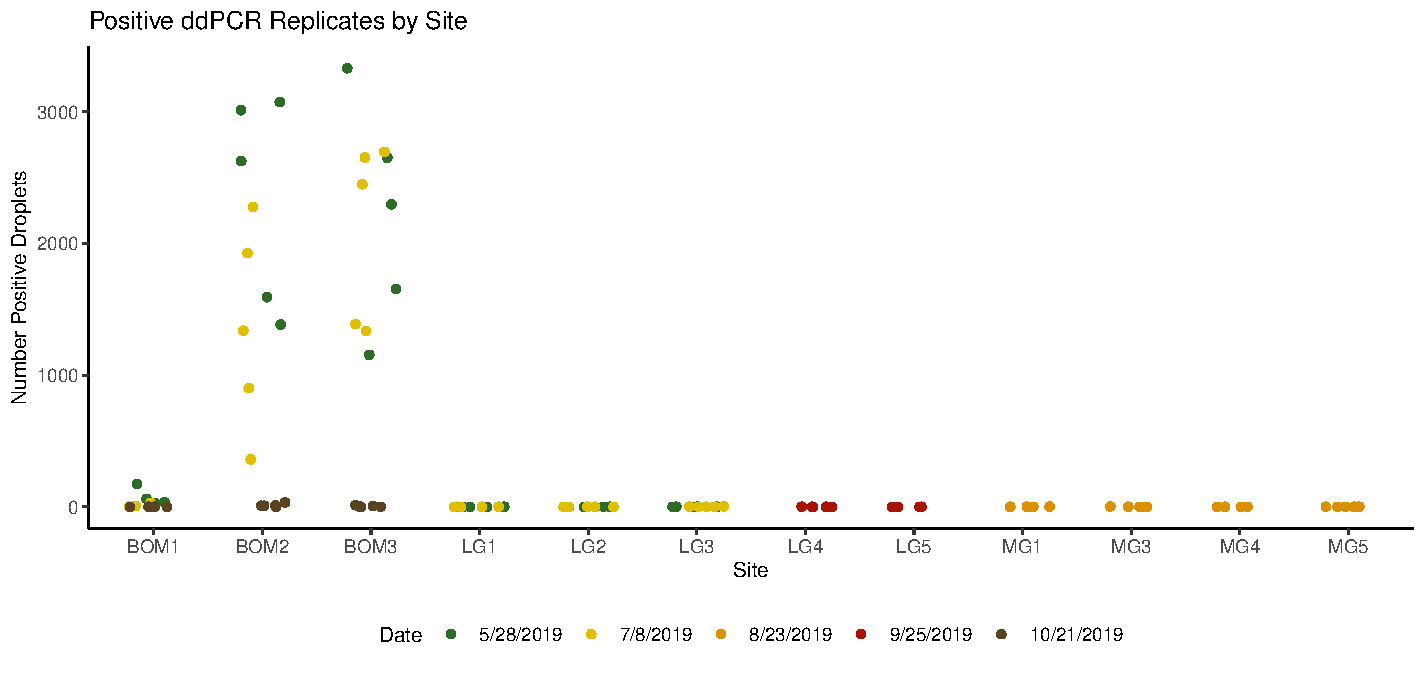
\includegraphics[width=\maxwidth]{figure/eDNA_visualization_droplets-1} 

}

\caption[A plot of the proportion of positive droplets from each sample by sampling site, colored by the date on which the sample was taken]{A plot of the proportion of positive droplets from each sample by sampling site, colored by the date on which the sample was taken.}\label{fig:eDNA_dropletseDNA_visualization_droplets}
\end{figure}


\end{knitrout}

\begin{knitrout}
\definecolor{shadecolor}{rgb}{0.969, 0.969, 0.969}\color{fgcolor}\begin{kframe}
\begin{alltt}
\hlstd{BOM} \hlkwb{<-} \hlstd{eDNA.df} \hlopt
  \hlkwd{filter}\hlstd{(Lake} \hlopt{==} \hlstr{"BOM"}\hlstd{)} \hlopt
  \hlkwd{ggplot}\hlstd{(}\hlkwd{aes}\hlstd{(}\hlkwc{x} \hlstd{= Site,}
             \hlkwc{y} \hlstd{= Positive.Droplets,}
             \hlkwc{colour} \hlstd{= Date.Collected))} \hlopt{+}
  \hlkwd{labs}\hlstd{(}\hlkwc{title} \hlstd{=} \hlstr{'Positive ddPCR Replicates at Lake BOM by Site'}\hlstd{,}
       \hlkwc{x} \hlstd{=} \hlstr{'Site'}\hlstd{,}
       \hlkwc{y} \hlstd{=} \hlstr{'Positive Droplets'}\hlstd{,}
       \hlkwc{color} \hlstd{=} \hlstr{'Date'}\hlstd{)} \hlopt{+}
  \hlkwd{geom_point}\hlstd{(}\hlkwc{position} \hlstd{=} \hlkwd{position_jitter}\hlstd{(}\hlkwc{width} \hlstd{=} \hlnum{0.25}\hlstd{,}
                                        \hlkwc{height} \hlstd{=} \hlnum{1}\hlstd{,}
                                        \hlkwc{seed} \hlstd{=} \hlnum{03172020}\hlstd{))} \hlopt{+}
  \hlkwd{scale_colour_manual}\hlstd{(}\hlkwc{values} \hlstd{= date.cols)} \hlopt{+}
  \hlkwd{theme_bw}\hlstd{()} \hlopt{+}
  \hlkwd{theme}\hlstd{(}\hlkwc{title} \hlstd{=} \hlkwd{element_text}\hlstd{(}\hlkwc{size} \hlstd{=} \hlnum{8}\hlstd{),}
        \hlkwc{panel.border} \hlstd{=} \hlkwd{element_blank}\hlstd{(),}
        \hlkwc{panel.grid.major} \hlstd{=} \hlkwd{element_blank}\hlstd{(),}
        \hlkwc{panel.grid.minor} \hlstd{=} \hlkwd{element_blank}\hlstd{(),}
        \hlkwc{axis.line} \hlstd{=} \hlkwd{element_line}\hlstd{(}\hlkwc{colour} \hlstd{=} \hlstr{"black"}\hlstd{),}
        \hlkwc{legend.position} \hlstd{=} \hlstr{'bottom'}\hlstd{)}


\hlstd{LG} \hlkwb{<-} \hlstd{eDNA.df} \hlopt
  \hlkwd{filter}\hlstd{(Lake} \hlopt{==} \hlstr{"LG"}\hlstd{)} \hlopt
  \hlkwd{ggplot}\hlstd{(}\hlkwd{aes}\hlstd{(}\hlkwc{x} \hlstd{= Site,}
             \hlkwc{y} \hlstd{= Positive.Droplets,}
             \hlkwc{colour} \hlstd{= Date.Collected))} \hlopt{+}
  \hlkwd{labs}\hlstd{(}\hlkwc{title} \hlstd{=} \hlstr{'Positive ddPCR Replicates at Lake LG by Site'}\hlstd{,}
       \hlkwc{x} \hlstd{=} \hlstr{'Site'}\hlstd{,}
       \hlkwc{y} \hlstd{=} \hlstr{'Positive Droplets'}\hlstd{,}
       \hlkwc{color} \hlstd{=} \hlstr{'Date'}\hlstd{)} \hlopt{+}
  \hlkwd{ylim}\hlstd{(}\hlkwd{c}\hlstd{(}\hlopt{-}\hlnum{0.01}\hlstd{,} \hlnum{3}\hlstd{))} \hlopt{+}
  \hlkwd{geom_point}\hlstd{(}\hlkwc{position} \hlstd{=} \hlkwd{position_jitter}\hlstd{(}\hlkwc{width} \hlstd{=} \hlnum{0.25}\hlstd{,}
                                        \hlkwc{height} \hlstd{=} \hlnum{0.001}\hlstd{,}
                                        \hlkwc{seed} \hlstd{=} \hlnum{03172020}\hlstd{))} \hlopt{+}
  \hlkwd{scale_colour_manual}\hlstd{(}\hlkwc{values} \hlstd{= date.cols)} \hlopt{+}
  \hlkwd{theme_bw}\hlstd{()} \hlopt{+}
  \hlkwd{theme}\hlstd{(}\hlkwc{title} \hlstd{=} \hlkwd{element_text}\hlstd{(}\hlkwc{size} \hlstd{=} \hlnum{8}\hlstd{),}
        \hlkwc{panel.border} \hlstd{=} \hlkwd{element_blank}\hlstd{(),}
        \hlkwc{panel.grid.major} \hlstd{=} \hlkwd{element_blank}\hlstd{(),}
        \hlkwc{panel.grid.minor} \hlstd{=} \hlkwd{element_blank}\hlstd{(),}
        \hlkwc{axis.line} \hlstd{=} \hlkwd{element_line}\hlstd{(}\hlkwc{colour} \hlstd{=} \hlstr{"black"}\hlstd{),}
        \hlkwc{legend.position} \hlstd{=} \hlstr{'bottom'}\hlstd{)}


\hlstd{MG} \hlkwb{<-} \hlstd{eDNA.df} \hlopt
  \hlkwd{filter}\hlstd{(Lake} \hlopt{==} \hlstr{"MG"}\hlstd{)} \hlopt
  \hlkwd{ggplot}\hlstd{(}\hlkwd{aes}\hlstd{(}\hlkwc{x} \hlstd{= Site,}
             \hlkwc{y} \hlstd{= Positive.Droplets,}
             \hlkwc{colour} \hlstd{= Date.Collected))} \hlopt{+}
  \hlkwd{labs}\hlstd{(}\hlkwc{title} \hlstd{=} \hlstr{'Positive ddPCR Replicates at Lake MG by Site'}\hlstd{,}
       \hlkwc{x} \hlstd{=} \hlstr{'Site'}\hlstd{,}
       \hlkwc{y} \hlstd{=} \hlstr{'Positive Droplets'}\hlstd{,}
       \hlkwc{color} \hlstd{=} \hlstr{'Date'}\hlstd{)} \hlopt{+}
  \hlkwd{ylim}\hlstd{(}\hlkwd{c}\hlstd{(}\hlopt{-}\hlnum{0.01}\hlstd{,} \hlnum{3}\hlstd{))} \hlopt{+}
  \hlkwd{geom_point}\hlstd{(}\hlkwc{position} \hlstd{=} \hlkwd{position_jitter}\hlstd{(}\hlkwc{width} \hlstd{=} \hlnum{0.25}\hlstd{,}
                                        \hlkwc{height} \hlstd{=} \hlnum{0.001}\hlstd{,}
                                        \hlkwc{seed} \hlstd{=} \hlnum{03172020}\hlstd{))} \hlopt{+}
  \hlkwd{scale_colour_manual}\hlstd{(}\hlkwc{values} \hlstd{= date.cols)} \hlopt{+}
  \hlkwd{theme_bw}\hlstd{()} \hlopt{+}
  \hlkwd{theme}\hlstd{(}\hlkwc{title} \hlstd{=} \hlkwd{element_text}\hlstd{(}\hlkwc{size} \hlstd{=} \hlnum{8}\hlstd{),}
        \hlkwc{panel.border} \hlstd{=} \hlkwd{element_blank}\hlstd{(),}
        \hlkwc{panel.grid.major} \hlstd{=} \hlkwd{element_blank}\hlstd{(),}
        \hlkwc{panel.grid.minor} \hlstd{=} \hlkwd{element_blank}\hlstd{(),}
        \hlkwc{axis.line} \hlstd{=} \hlkwd{element_line}\hlstd{(}\hlkwc{colour} \hlstd{=} \hlstr{"black"}\hlstd{),}
        \hlkwc{legend.position} \hlstd{=} \hlstr{'bottom'}\hlstd{)}


\hlkwd{grid.arrange}\hlstd{(BOM, LG, MG,} \hlkwc{ncol} \hlstd{=} \hlnum{3}\hlstd{)}
\end{alltt}
\end{kframe}
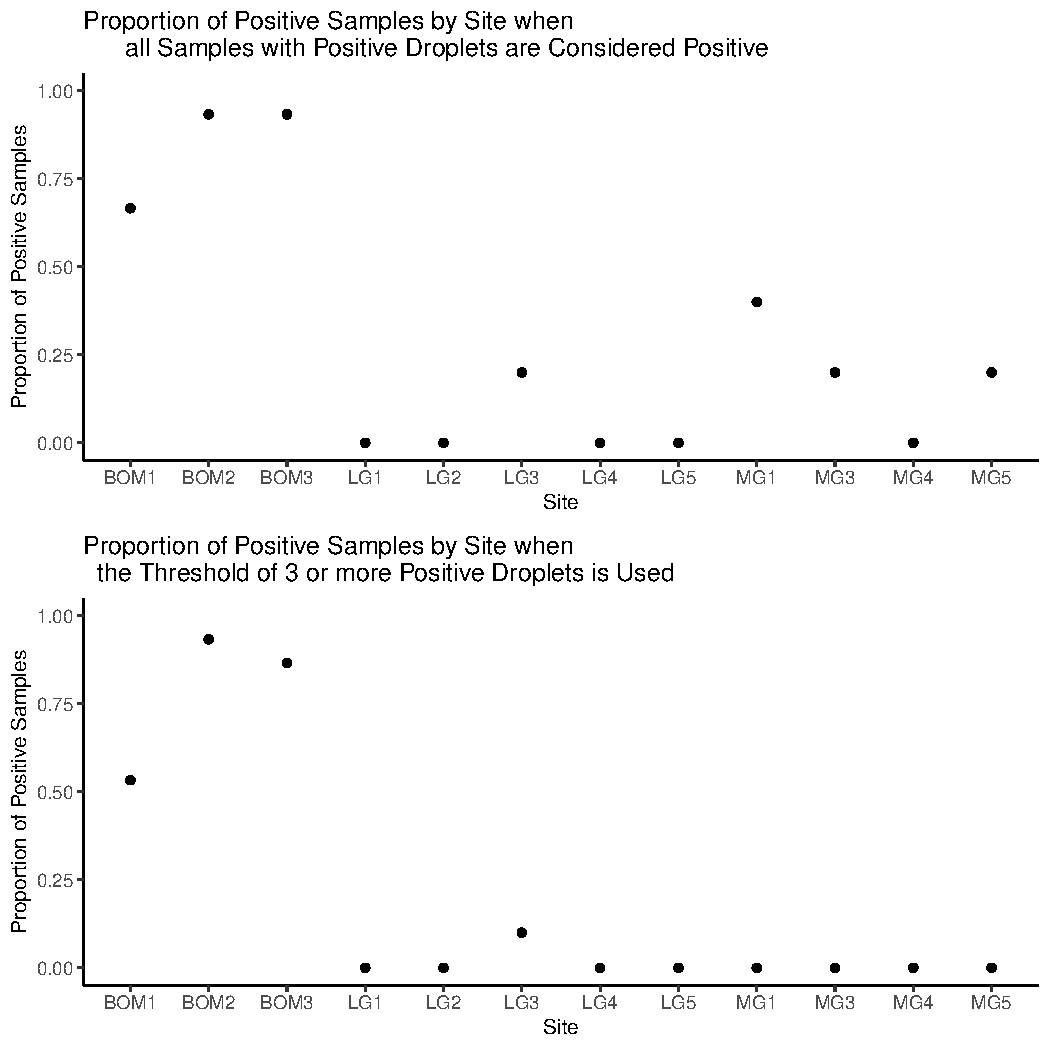
\includegraphics[width=\maxwidth]{figure/unnamed-chunk-1-1} 

\end{knitrout}

\subsection{Plankton Tow Survey Data}

Plankton tow data description
\begin{itemize}
  \item data source: BOR
  \item region
  \item number of lakes (number of lakes where dreissenid mussel veligers were detected)
  \item number of sites
  \item dates
  \item potential covariates
\end{itemize}

\begin{figure}[h]
	\centering
	
\includegraphics[scale = 0.7]{planktontow}
	\caption{A diagram displaying the structure of the plankton tow data.}
	\label{pt}
\end{figure}

Plankton tow data visualization

\section{Methods}

\subsection{Bayesian Modeling Background}

\subsection{Occupancy Models}

\textbf{this is still in the works}

Occupancy is the presence of a particular species on a given site, this may not be the first choice of state variables to ecologists but occupancy studies are useful when there is a large spatial scale or the study is conducted over many years, when abundance or vital rates are hard to measure. Occupancy studies are also useful over capture-recapture methods when individuals cannot be marked or uniquely identified. However, sometimes patterns of species occurrence are of interest, this happens when researchers are interested in the range of a species or the spread of invasion. The sampling units for occupancy studies are called 'sites'. We can learn about detection probabilities when multiple site visits are used. Also, when using occupancy models we need to account for imperfect detection because it is possible that the researchers could miss the species even if it is present at the site. 

Hierarchical structure of eDNA data creates dependencies that need to be accounted for \cite{MacKenzie}

in the hierarchical multi-scale occupancy model (with three nested levels) defined by \cite{Dorazio_Erickson}:
\begin{itemize}
\item learn about the probability of species occurrence at a site 
\item $Z_i$ denotes the presence or absence of the target species at the $i^{th}$ site ($i = 1, \dots, M$)
\item $Z_i \sim Bernoulli(\psi_i)$
\item $\psi_i$ is the probability that the target species is present at the $i^{th}$ site
\item $\bm{\beta}$ are the site level regression parameters for $\psi_i$
\item $\bm{x}_i$ are the site level covariates for $\psi_i$
\item learn about the conditional probability of species occurrence in a sample of a site given the species is present at the site
\item $A_{ij}$ denotes the presence or absence of the target species in the $j^{th}$ sample from the $i^{th}$ site ($j = 1, \dots, J_i$)
\item $A_{ij}|z_i \sim Bernoulli(z_i\theta_{ij})$
\item $z_i$ is a realized value of $Z_i$
\item $\theta_{ij}$ is the conditional probability that the target species is present in the $j^{th}$ sample from the $i^{th}$ site, given the target species is present at the location 
\item $\bm{\alpha}$ are the sample level regression parameters for $\theta_{ij}$
\item $\bm{w}_{ij}$ are the sample level covariates for $\theta_{ij}$
\item learn about the conditional probability of detection of the species in a sub-sample of a sample given that the species is present in the sample
\item $Y_{ijk}$ denotes the detected or not detected in the $k^{th}$ replicate of the $j^{th}$ sample collected at the $i^{th}$ site ($k = 1, \dots, K_{ij}$)
\item $Y_{ijk}|a_{ij} \sim Bernoulli(a_{ij}p_{ijk})$
\item $a_{ij}$ is a realized value of $A_{ij}$
\item $p_{ijk}$ denotes the probability that the target species is detected in the $k^{th}$ replicate of the $j^{th}$ sample collected at the $i^{th}$ site, given the target species is present in that sample
\item if $p_{ijk}$ does not differ among the replicates, and the replicates are independent, then $Y_{ij} = \sum_{k = 1}^{K_{ij}}Y_{ijk}$
\item $Y_{ij}|a_{ij} \sim Binomial(K_{ij}, a_{ij}p_{ij})$
\item $p_{ij}$ is the conditional probability of detection of the target species in each replicate of the $j^{th}$ sample collected at the $i^th$ location, given that the target species is present in that sample
\item $\bm{\delta}$ are the sample level regression parameters for $p_{ij}$ 
\item $\bm{v}_{ij}$ are the sample level covariates for $p_{ij}$
\end{itemize}

The assumptions are: 
\begin{itemize}
\item The species is not misidentified, no false positives
\item no un-modeled heterogeneity in the probabilities of detection and occupancy
\item each survey is closed to changes in occupancy over the sampling period
\item the detection of the species is independent for each survey
\end{itemize}


In WILD 502 when talking about multi-season occupancy models, we talked about extirpation and colonization rates, but I think that these could be modeled with a latent variable(s)? I don't think they are of particular interest here. 






 
\subsection{Implementation}

Package options for Multi-season (should we even be using these models or should we be modeling the time component in another way) single-species occupancy models: 
\begin{itemize}
\item nimble.dynamic.occ
\item STAN
\item JAGS
\item wiquid package??
\item Frequentist Options: 
  \begin{itemize}
  \item unmarked
  \item Program MARK
  \end{itemize}
\item write my own package? 
\end{itemize}

Package for eDNA data: 

\texttt{msocc} package

\section{Analysis}

\subsection{Analysis of eDNA Data}

analysis and results



\begin{knitrout}
\definecolor{shadecolor}{rgb}{0.969, 0.969, 0.969}\color{fgcolor}\begin{kframe}
\begin{alltt}
\hlstd{eDNA_m1} \hlkwb{<-} \hlkwd{msocc_mod}\hlstd{(eDNA_wide,}
                     \hlkwc{site} \hlstd{=} \hlkwd{list}\hlstd{(}\hlkwc{model} \hlstd{=} \hlopt{~} \hlnum{1}\hlstd{,} \hlkwc{cov_tbl} \hlstd{= site.cov),}
                     \hlkwc{sample} \hlstd{=} \hlkwd{list}\hlstd{(}\hlkwc{model} \hlstd{=} \hlopt{~} \hlnum{1}\hlstd{,} \hlkwc{cov_tbl} \hlstd{= sample.cov),}
                     \hlkwc{rep} \hlstd{=} \hlkwd{list}\hlstd{(}\hlkwc{model} \hlstd{=} \hlopt{~} \hlnum{1}\hlstd{,} \hlkwc{cov_tbl} \hlstd{= rep.cov),}
                     \hlkwc{seed} \hlstd{=} \hlnum{03202020}\hlstd{)}

\hlstd{burnin} \hlkwb{<-} \hlnum{100}

\hlcom{# site summary}
\hlcom{## posterior_summary function does not work b/c matrix too large }
\hlstd{psi.post_m1} \hlkwb{<-} \hlstd{eDNA_m1}\hlopt{$}\hlstd{psi[}\hlopt{-}\hlstd{(}\hlnum{1}\hlopt{:}\hlstd{burnin)]}
\hlkwd{summary}\hlstd{(psi.post_m1)}
\hlkwd{quantile}\hlstd{(psi.post_m1,} \hlkwd{c}\hlstd{(}\hlnum{0.025}\hlstd{,} \hlnum{0.975}\hlstd{))}
\hlkwd{plot}\hlstd{(psi.post_m1,} \hlkwc{type} \hlstd{=} \hlstr{"l"}\hlstd{)} \hlcom{# REDO THIS IN GGPLOT IF KEEPING IT}

\hlcom{# sample summary}
\hlcom{## posterior_summary function does not work b/c matrix too large}
\hlstd{theta.post_m1} \hlkwb{<-} \hlstd{eDNA_m1}\hlopt{$}\hlstd{theta[}\hlopt{-}\hlstd{(}\hlnum{1}\hlopt{:}\hlstd{burnin)]}
\hlkwd{summary}\hlstd{(theta.post_m1)}
\hlkwd{quantile}\hlstd{(theta.post_m1,} \hlkwd{c}\hlstd{(}\hlnum{0.025}\hlstd{,} \hlnum{0.975}\hlstd{))}
\hlkwd{plot}\hlstd{(theta.post_m1,} \hlkwc{type} \hlstd{=} \hlstr{"l"}\hlstd{)} \hlcom{# REDO THIS IN GGPLOT IF KEEPING IT}

\hlcom{# rep summary}
\hlcom{## posterior_summary function does not work b/c matrix too large}
\hlstd{p.post_m1} \hlkwb{<-} \hlstd{eDNA_m1}\hlopt{$}\hlstd{p[}\hlopt{-}\hlstd{(}\hlnum{1}\hlopt{:}\hlstd{burnin)]}
\hlkwd{summary}\hlstd{(p.post_m1)}
\hlkwd{quantile}\hlstd{(p.post_m1,} \hlkwd{c}\hlstd{(}\hlnum{0.025}\hlstd{,} \hlnum{0.975}\hlstd{))}
\hlkwd{plot}\hlstd{(p.post_m1,} \hlkwc{type} \hlstd{=} \hlstr{"l"}\hlstd{)} \hlcom{# REDO THIS IN GGPLOT IF KEEPING IT}
\end{alltt}
\end{kframe}
\end{knitrout}

\begin{knitrout}
\definecolor{shadecolor}{rgb}{0.969, 0.969, 0.969}\color{fgcolor}\begin{kframe}
\begin{alltt}
\hlstd{eDNA_m2} \hlkwb{<-} \hlkwd{msocc_mod}\hlstd{(eDNA_wide,}
                     \hlkwc{site} \hlstd{=} \hlkwd{list}\hlstd{(}\hlkwc{model} \hlstd{=} \hlopt{~} \hlstd{lake,} \hlkwc{cov_tbl} \hlstd{= site.cov),}
                     \hlkwc{sample} \hlstd{=} \hlkwd{list}\hlstd{(}\hlkwc{model} \hlstd{=} \hlopt{~} \hlstd{date,} \hlkwc{cov_tbl} \hlstd{= sample.cov),}
                     \hlkwc{rep} \hlstd{=} \hlkwd{list}\hlstd{(}\hlkwc{model} \hlstd{=} \hlopt{~} \hlnum{1}\hlstd{,} \hlkwc{cov_tbl} \hlstd{= rep.cov),}
                     \hlkwc{seed} \hlstd{=} \hlnum{03202020}\hlstd{)}

\hlstd{burnin} \hlkwb{<-} \hlnum{100}



\hlcom{# site summary}
\hlcom{## posterior_summary function does not work b/c matrix too large}
\hlstd{X} \hlkwb{<-} \hlstd{eDNA_m2}\hlopt{$}\hlstd{model.info}\hlopt{$}\hlstd{X}
\hlstd{beta} \hlkwb{<-} \hlstd{eDNA_m2}\hlopt{$}\hlstd{beta}

\hlstd{eta} \hlkwb{<-} \hlstd{beta} \hlopt \hlkwd{t}\hlstd{(X)}
\hlstd{psi} \hlkwb{<-} \hlkwd{exp}\hlstd{(eta)}\hlopt{/}\hlstd{(}\hlnum{1} \hlopt{+} \hlkwd{exp}\hlstd{(eta))}

\hlstd{psi.mcmc} \hlkwb{<-} \hlstd{psi[}\hlopt{-}\hlkwd{c}\hlstd{(}\hlnum{1}\hlopt{:}\hlstd{burnin), ]}

\hlstd{mean} \hlkwb{<-} \hlkwd{apply}\hlstd{(psi.mcmc,} \hlnum{2}\hlstd{, mean)}
\hlstd{median} \hlkwb{<-} \hlkwd{apply}\hlstd{(psi.mcmc,} \hlnum{2}\hlstd{, median)}
\hlstd{quantiles} \hlkwb{<-} \hlkwd{apply}\hlstd{(psi.mcmc,} \hlnum{2}\hlstd{, quantile,} \hlkwc{probs} \hlstd{=} \hlkwd{c}\hlstd{(}\hlnum{0.025}\hlstd{,} \hlnum{0.975}\hlstd{))}
\hlstd{sum_tbl} \hlkwb{<-} \hlstd{eDNA_m2}\hlopt{$}\hlstd{model.info}\hlopt{$}\hlstd{df} \hlopt
  \hlstd{dplyr}\hlopt{::}\hlkwd{select}\hlstd{(}\hlopt{-}\hlstd{sample,} \hlopt{-}\hlstd{rep)} \hlopt
  \hlstd{dplyr}\hlopt{::}\hlkwd{distinct}\hlstd{()} \hlopt
  \hlstd{dplyr}\hlopt{::}\hlkwd{mutate}\hlstd{(}\hlkwc{median} \hlstd{= median,}
                \hlkwc{mean} \hlstd{= mean,}
                \hlkwc{lwr} \hlstd{= quantiles[}\hlnum{1}\hlstd{, ],}
                \hlkwc{upr} \hlstd{= quantiles[}\hlnum{2}\hlstd{, ])}
\hlstd{sum_tbl}

\hlcom{# sample summary}
\hlcom{## posterior_summary function does not work b/c matrix too large}
\hlcom{### theta.post_m2 }
\hlstd{W} \hlkwb{<-} \hlstd{eDNA_m2}\hlopt{$}\hlstd{model.info}\hlopt{$}\hlstd{W}
\hlstd{alpha} \hlkwb{<-} \hlstd{eDNA_m2}\hlopt{$}\hlstd{alpha}

\hlstd{nu} \hlkwb{<-} \hlstd{alpha} \hlopt \hlkwd{t}\hlstd{(W)}
\hlstd{theta} \hlkwb{<-} \hlkwd{exp}\hlstd{(nu)}\hlopt{/}\hlstd{(}\hlnum{1} \hlopt{+} \hlkwd{exp}\hlstd{(nu))}

\hlstd{theta.mcmc} \hlkwb{<-} \hlstd{theta[}\hlopt{-}\hlkwd{c}\hlstd{(}\hlnum{1}\hlopt{:}\hlstd{burnin), ]}

\hlstd{mean} \hlkwb{<-} \hlkwd{apply}\hlstd{(theta.mcmc,} \hlnum{2}\hlstd{, mean)}
\hlstd{median} \hlkwb{<-} \hlkwd{apply}\hlstd{(theta.mcmc,} \hlnum{2}\hlstd{, median)}
\hlstd{quantiles} \hlkwb{<-} \hlkwd{apply}\hlstd{(theta.mcmc,} \hlnum{2}\hlstd{, quantile,} \hlkwc{probs} \hlstd{=} \hlkwd{c}\hlstd{(}\hlnum{0.025}\hlstd{,} \hlnum{0.975}\hlstd{))}
\hlstd{sum_tbl} \hlkwb{<-} \hlstd{eDNA_m2}\hlopt{$}\hlstd{model.info}\hlopt{$}\hlstd{df} \hlopt \hlstd{dplyr}\hlopt{::}\hlkwd{select}\hlstd{(}\hlopt{-}\hlstd{rep)} \hlopt
  \hlstd{dplyr}\hlopt{::}\hlkwd{distinct}\hlstd{()} \hlopt
  \hlstd{dplyr}\hlopt{::}\hlkwd{mutate}\hlstd{(}\hlkwc{median} \hlstd{= median,}
                \hlkwc{mean} \hlstd{= mean,}
                \hlkwc{lwr} \hlstd{= quantiles[}\hlnum{1}\hlstd{, ],}
                \hlkwc{upr} \hlstd{= quantiles[}\hlnum{2}\hlstd{, ])}
\hlstd{sum_tbl}

\hlcom{# rep summary}
\hlcom{## posterior_summary function does not work b/c matrix too large}
\hlstd{p.post_m2} \hlkwb{<-} \hlstd{eDNA_m2}\hlopt{$}\hlstd{p[}\hlopt{-}\hlstd{(}\hlnum{1}\hlopt{:}\hlstd{burnin)]}
\hlkwd{summary}\hlstd{(p.post_m2)}
\hlkwd{quantile}\hlstd{(p.post_m2,} \hlkwd{c}\hlstd{(}\hlnum{0.025}\hlstd{,} \hlnum{0.975}\hlstd{))}
\hlkwd{plot}\hlstd{(p.post_m2,} \hlkwc{type} \hlstd{=} \hlstr{"l"}\hlstd{)} \hlcom{# REDO THIS IN GGPLOT IF KEEPING IT}
\end{alltt}
\end{kframe}
\end{knitrout}

\begin{knitrout}
\definecolor{shadecolor}{rgb}{0.969, 0.969, 0.969}\color{fgcolor}\begin{kframe}
\begin{alltt}
\hlstd{eDNA_m3} \hlkwb{<-} \hlkwd{msocc_mod}\hlstd{(eDNA_wide,}
                     \hlkwc{site} \hlstd{=} \hlkwd{list}\hlstd{(}\hlkwc{model} \hlstd{=} \hlopt{~} \hlstd{site,} \hlkwc{cov_tbl} \hlstd{= site.cov),}
                     \hlkwc{sample} \hlstd{=} \hlkwd{list}\hlstd{(}\hlkwc{model} \hlstd{=} \hlopt{~} \hlnum{1}\hlstd{,} \hlkwc{cov_tbl} \hlstd{= sample.cov),}
                     \hlkwc{rep} \hlstd{=} \hlkwd{list}\hlstd{(}\hlkwc{model} \hlstd{=} \hlopt{~} \hlnum{1}\hlstd{,} \hlkwc{cov_tbl} \hlstd{= rep.cov),}
                     \hlkwc{seed} \hlstd{=} \hlnum{03202020}\hlstd{)}

\hlstd{burnin} \hlkwb{<-} \hlnum{100}



\hlcom{# site summary}
\hlcom{## posterior_summary function does not work b/c matrix too large}
\hlstd{X} \hlkwb{<-} \hlstd{eDNA_m3}\hlopt{$}\hlstd{model.info}\hlopt{$}\hlstd{X}
\hlstd{beta} \hlkwb{<-} \hlstd{eDNA_m3}\hlopt{$}\hlstd{beta}

\hlstd{eta} \hlkwb{<-} \hlstd{beta} \hlopt \hlkwd{t}\hlstd{(X)}
\hlstd{psi} \hlkwb{<-} \hlkwd{exp}\hlstd{(eta)}\hlopt{/}\hlstd{(}\hlnum{1} \hlopt{+} \hlkwd{exp}\hlstd{(eta))}

\hlstd{psi.mcmc} \hlkwb{<-} \hlstd{psi[}\hlopt{-}\hlkwd{c}\hlstd{(}\hlnum{1}\hlopt{:}\hlstd{burnin), ]}

\hlstd{mean} \hlkwb{<-} \hlkwd{apply}\hlstd{(psi.mcmc,} \hlnum{2}\hlstd{, mean)}
\hlstd{median} \hlkwb{<-} \hlkwd{apply}\hlstd{(psi.mcmc,} \hlnum{2}\hlstd{, median)}
\hlstd{quantiles} \hlkwb{<-} \hlkwd{apply}\hlstd{(psi.mcmc,} \hlnum{2}\hlstd{, quantile,} \hlkwc{probs} \hlstd{=} \hlkwd{c}\hlstd{(}\hlnum{0.025}\hlstd{,} \hlnum{0.975}\hlstd{))}
\hlstd{sum_tbl} \hlkwb{<-} \hlstd{eDNA_m3}\hlopt{$}\hlstd{model.info}\hlopt{$}\hlstd{df} \hlopt
  \hlstd{dplyr}\hlopt{::}\hlkwd{select}\hlstd{(}\hlopt{-}\hlstd{sample,} \hlopt{-}\hlstd{rep)} \hlopt
  \hlstd{dplyr}\hlopt{::}\hlkwd{distinct}\hlstd{()} \hlopt
  \hlstd{dplyr}\hlopt{::}\hlkwd{mutate}\hlstd{(}\hlkwc{median} \hlstd{= median,}
                \hlkwc{mean} \hlstd{= mean,}
                \hlkwc{lwr} \hlstd{= quantiles[}\hlnum{1}\hlstd{, ],}
                \hlkwc{upr} \hlstd{= quantiles[}\hlnum{2}\hlstd{, ])}
\hlstd{sum_tbl}
\end{alltt}
\end{kframe}
\end{knitrout}


\subsection{Analysis of Plankton Tow Data}

analysis and results 

\section{Discussion}

\subsection{Further Investigations}

\newpage
\section{References}
\begingroup
\renewcommand{\section}[2]{}%
\begin{flushleft}
\bibliographystyle{apalike}
%\bibliographystyle{acm}
%\bibliographystyle{abbrvnat}
%\bibliographystyle{unsrtnat}
%\bibliographystyle{ACM-Reference-Format}
\bibliography{bibliography}
\end{flushleft}
\endgroup

\newpage
\section{Appendix - R Code}

Things to think about for the simulation or questions I have: 
\begin{itemize}
\item think about how changing the detection probabilities and occupancy probabilities impact the results: 
	\begin{itemize}
	\item High occupancy, high detection
	\item High occupancy, low detection 
	\item Low occupancy, high detection 
	\item Low occupancy, low detection 
	\end{itemize}
\item How do we/can we include sample level covariates to account for sampling effort (number of tows, if available)?
\item If we are getting more data:
	\begin{itemize}
	\item How do we account for multiple sampling seasons (years)? 
	\item How do the assumptions of occupancy models change when we have several sampling years versus only 1
\end{itemize}
\end{itemize}

Additional questions, not directly related to the simulation:
\begin{itemize}
	\item How do we account for this multilevel (for lack of a better word) testing process? For example, sometimes (?) when they find them in the microscope, then they test them using polymerase chain reaction (PCR) to confirm positive identification, and sometimes gene sequencing (? -- looks like it was only used on one observation in the sample data), or scanning electron microscopy (SEM).
\end{itemize}

\singlespacing

\begin{knitrout}
\definecolor{shadecolor}{rgb}{0.969, 0.969, 0.969}\color{fgcolor}\begin{kframe}
\begin{verbatim}
# packages used 
library(car)
library(dplyr)
library(tidyr)
library(kableExtra)
library(ggplot2)
library(gridExtra)
library(tm)
## library(devtools)
## devtools::install_github("StrattonCh/msocc")
library(msocc)


# load eDNA data
eDNA <- read.csv(
  "C:/Users/mwind/OneDrive/Writing Project_EXTRA/eDNA.csv")


# rename lakes
levels(eDNA$Lake) <- c("BOM", "LG", "MG")


# remove field blank samples
eDNA <- eDNA %>% 
  filter(Site != "tb")
eDNA$Site <- droplevels(eDNA$Site)


# number of samples with (0, 3) positive droplets
eDNA %>% 
  count(Positive.Droplets < 3 & Positive.Droplets > 0)


# number of samples with 0 positive droplets
eDNA %>% 
  group_by(Lake) %>%
  count(Positive.Droplets == 0)


# reorder dates in chronological order
eDNA$Date.Collected <- factor(eDNA$Date.Collected,
                          levels = c("5/28/2019", "7/8/2019", 
                                     "8/23/2019", "9/25/2019",
                                     "10/21/2019"))


# generate table of 10 sample rows of eDNA data
set.seed(03142020)
knitr::kable(some(eDNA), 'latex', booktabs = T, linesep = "",
             caption = "\\label{tab:eDNA_data}10 sample rows of the eDNA data.", 
             align = 'c', row.names = F, 
             col.names = c("Lake", "Site", "Sample", "Date", "Water Temperature", 
                           "Concentration", "Positive Droplets")) %>%
  kable_styling(latex_options = 
                  c("scale_down", "hold_position"))


# BOM
eDNA %>% filter(Lake == "BOM") %>% summary

# LG
eDNA %>% filter(Lake == "LG") %>% summary

# MG
eDNA %>% filter(Lake == "MG") %>% summary


# visualization of eDNA data
eDNA.df <- data.frame(eDNA)

date.cols <- c("5/28/2019" = "#2d6b28", 
               "7/8/2019" = "#dfbf00",
               "8/23/2019" = "#db9002",
               "9/25/2019" = "#a91303",
               "10/21/2019" = "#5a4320")

eDNA.df %>% 
  ggplot(aes(x = Site, 
             y = Positive.Droplets/20000, 
             colour = Date.Collected)) + 
  labs(title = 'Proportion of Positive ddPCR Replicates by Site', 
       x = 'Site', 
       y = 'Proportion of Positive Droplets', 
       color = 'Date') +
  ylim(c(0, 1)) + 
  geom_point(position = position_jitter(width = 0.25, 
                                        height = 0.001, 
                                        seed = 03172020)) + 
  scale_colour_manual(values = date.cols) + 
  theme_bw() + 
  theme(title = element_text(size = 8),
        panel.border = element_blank(), 
        panel.grid.major = element_blank(),
        panel.grid.minor = element_blank(), 
        axis.line = element_line(colour = "black"), 
        legend.position = 'bottom')
\end{verbatim}
\end{kframe}
\end{knitrout}


\lstset{
	basicstyle=\ttfamily\scriptsize,
	columns=fullflexible,
	frame=single,
	breaklines=true,
	postbreak=\mbox{\textcolor{red}{$\hookrightarrow$}\space},
	keepspaces = TRUE,
}
%\begin{lstlisting}
%\end{lstlisting}
\end{document}
              
